\documentclass{standalone}
\usepackage{tikz}
\usetikzlibrary{patterns, positioning}


\begin{document}
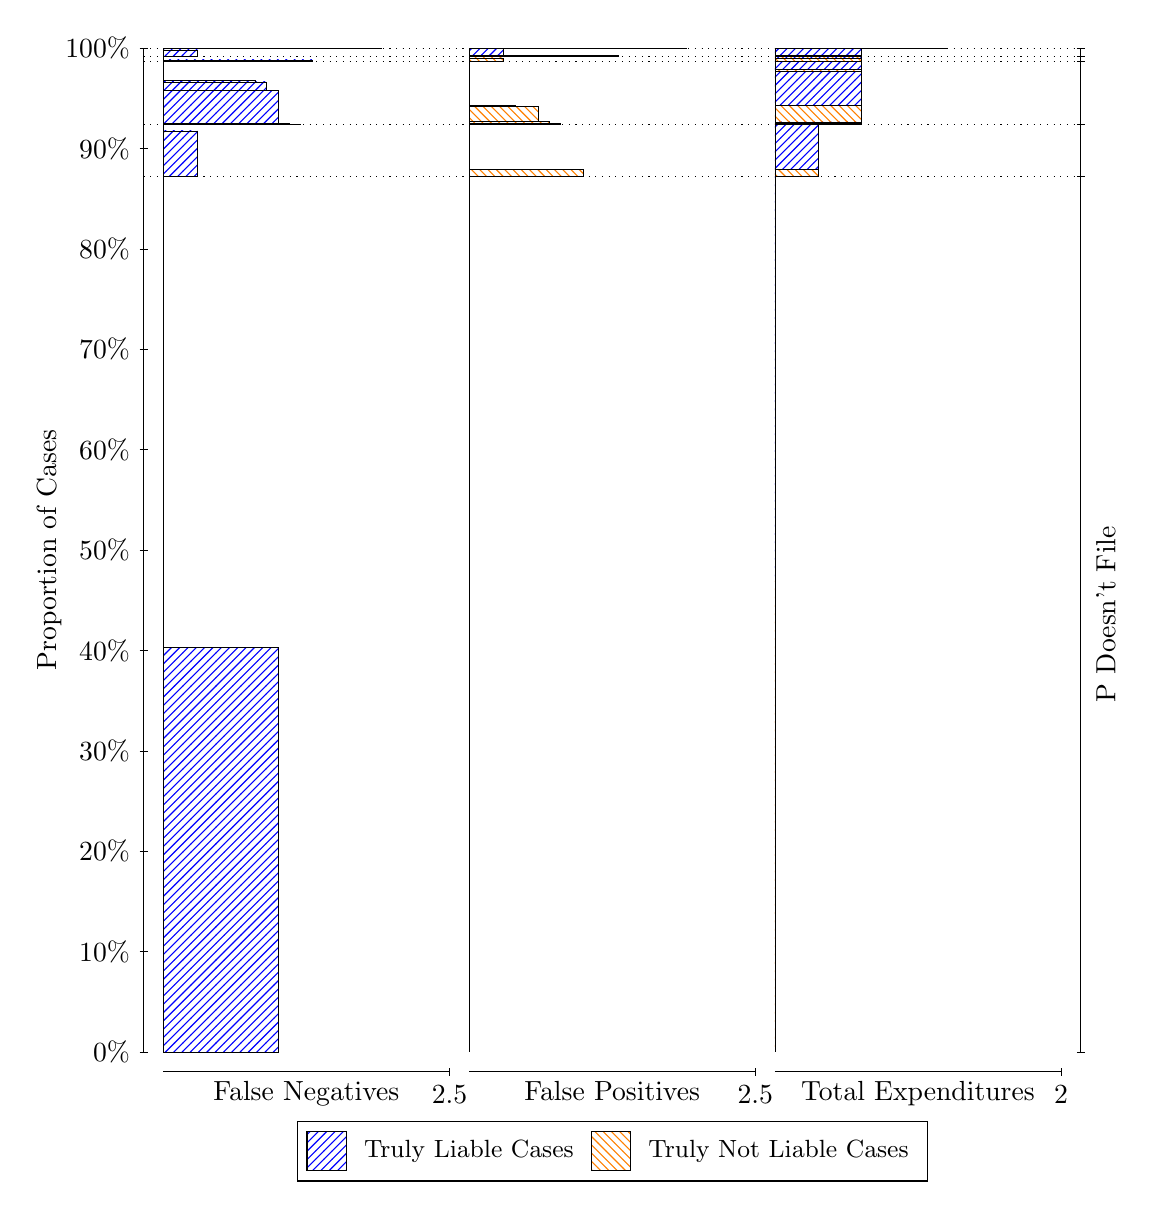
\begin{tikzpicture}
\draw[black, very thin] (1.5,1.75) -- (1.5,14.5);
\node[rotate=90, text=black, anchor=center] at (0.3, 8.125) {Proportion of Cases};
\draw[black, very thin] (1.45,1.75) -- (1.55,1.75);
\node[text=black, anchor=east] at (1.45, 1.75) {0\%};
\draw[black, very thin] (1.45,3.025) -- (1.55,3.025);
\node[text=black, anchor=east] at (1.45, 3.025) {10\%};
\draw[black, very thin] (1.45,4.3) -- (1.55,4.3);
\node[text=black, anchor=east] at (1.45, 4.3) {20\%};
\draw[black, very thin] (1.45,5.575) -- (1.55,5.575);
\node[text=black, anchor=east] at (1.45, 5.575) {30\%};
\draw[black, very thin] (1.45,6.85) -- (1.55,6.85);
\node[text=black, anchor=east] at (1.45, 6.85) {40\%};
\draw[black, very thin] (1.45,8.125) -- (1.55,8.125);
\node[text=black, anchor=east] at (1.45, 8.125) {50\%};
\draw[black, very thin] (1.45,9.4) -- (1.55,9.4);
\node[text=black, anchor=east] at (1.45, 9.4) {60\%};
\draw[black, very thin] (1.45,10.675) -- (1.55,10.675);
\node[text=black, anchor=east] at (1.45, 10.675) {70\%};
\draw[black, very thin] (1.45,11.95) -- (1.55,11.95);
\node[text=black, anchor=east] at (1.45, 11.95) {80\%};
\draw[black, very thin] (1.45,13.225) -- (1.55,13.225);
\node[text=black, anchor=east] at (1.45, 13.225) {90\%};
\draw[black, very thin] (1.45,14.5) -- (1.55,14.5);
\node[text=black, anchor=east] at (1.45, 14.5) {100\%};

\draw[black, very thin] (13.4,1.75) -- (13.4,14.5);
\draw[black, very thin] (13.35,1.75) -- (13.45,1.75);
\node[anchor=west] at (13.35, 1.75) {};
\draw[black, very thin] (13.35,12.871) -- (13.45,12.871);
\node[anchor=west] at (13.35, 12.871) {};
\draw[black, very thin] (13.35,13.531) -- (13.45,13.531);
\node[anchor=west] at (13.35, 13.531) {};
\draw[black, very thin] (13.35,14.331) -- (13.45,14.331);
\node[anchor=west] at (13.35, 14.331) {};
\draw[black, very thin] (13.35,14.393) -- (13.45,14.393);
\node[anchor=west] at (13.35, 14.393) {};
\draw[black, very thin] (13.35,14.495) -- (13.45,14.495);
\node[anchor=west] at (13.35, 14.495) {};
\draw[black, very thin] (13.35,14.497) -- (13.45,14.497);
\node[anchor=west] at (13.35, 14.497) {};
\draw[black, very thin] (13.35,14.5) -- (13.45,14.5);
\node[anchor=west] at (13.35, 14.5) {};

\draw[black, very thin, pattern color=blue, pattern=north east lines] (1.75,1.75) rectangle (3.2033,6.8879);
\draw[black, very thin, pattern color=orange, pattern=north west lines] (1.75,6.8879) rectangle (1.75,12.871);
\draw[black, very thin, pattern color=blue, pattern=north east lines] (1.75,12.871) rectangle (2.186,13.448);
\draw[black, very thin, pattern color=orange, pattern=north west lines] (1.75,13.448) rectangle (1.75,13.531);
\draw[black, very thin, pattern color=blue, pattern=north east lines] (1.75,13.531) rectangle (3.494,13.535);
\draw[black, very thin, pattern color=blue, pattern=north east lines] (1.75,13.535) rectangle (3.3487,13.539);
\draw[black, very thin, pattern color=blue, pattern=north east lines] (1.75,13.539) rectangle (3.2033,13.962);
\draw[black, very thin, pattern color=blue, pattern=north east lines] (1.75,13.962) rectangle (3.058,14.069);
\draw[black, very thin, pattern color=blue, pattern=north east lines] (1.75,14.069) rectangle (2.9127,14.086);
\draw[black, very thin, pattern color=orange, pattern=north west lines] (1.75,14.086) rectangle (1.75,14.331);
\draw[black, very thin, pattern color=blue, pattern=north east lines] (1.75,14.331) rectangle (3.6393,14.349);
\draw[black, very thin, pattern color=orange, pattern=north west lines] (1.75,14.349) rectangle (1.75,14.393);
\draw[black, very thin, pattern color=blue, pattern=north east lines] (1.75,14.393) rectangle (2.186,14.477);
\draw[black, very thin, pattern color=orange, pattern=north west lines] (1.75,14.477) rectangle (1.75,14.495);
\draw[black, very thin, pattern color=blue, pattern=north east lines] (1.75,14.495) rectangle (4.5113,14.496);
\draw[black, very thin, pattern color=orange, pattern=north west lines] (1.75,14.496) rectangle (1.75,14.497);
\draw[black, very thin, pattern color=blue, pattern=north east lines] (1.75,14.497) rectangle (2.186,14.499);
\draw[black, very thin, pattern color=orange, pattern=north west lines] (1.75,14.499) rectangle (1.75,14.5);
\draw[black, very thin, pattern color=orange, pattern=north west lines] (5.6333,1.75) rectangle (5.6333,7.7326);
\draw[black, very thin, pattern color=blue, pattern=north east lines] (5.6333,7.7326) rectangle (5.6333,12.871);
\draw[black, very thin, pattern color=orange, pattern=north west lines] (5.6333,12.871) rectangle (7.0867,12.954);
\draw[black, very thin, pattern color=blue, pattern=north east lines] (5.6333,12.954) rectangle (5.6333,13.531);
\draw[black, very thin, pattern color=orange, pattern=north west lines] (5.6333,13.531) rectangle (6.796,13.545);
\draw[black, very thin, pattern color=orange, pattern=north west lines] (5.6333,13.545) rectangle (6.6507,13.57);
\draw[black, very thin, pattern color=orange, pattern=north west lines] (5.6333,13.57) rectangle (6.5053,13.761);
\draw[black, very thin, pattern color=orange, pattern=north west lines] (5.6333,13.761) rectangle (6.36,13.763);
\draw[black, very thin, pattern color=orange, pattern=north west lines] (5.6333,13.763) rectangle (6.2147,13.776);
\draw[black, very thin, pattern color=blue, pattern=north east lines] (5.6333,13.776) rectangle (5.6333,14.331);
\draw[black, very thin, pattern color=orange, pattern=north west lines] (5.6333,14.331) rectangle (6.0693,14.375);
\draw[black, very thin, pattern color=blue, pattern=north east lines] (5.6333,14.375) rectangle (5.6333,14.393);
\draw[black, very thin, pattern color=orange, pattern=north west lines] (5.6333,14.393) rectangle (7.5227,14.411);
\draw[black, very thin, pattern color=blue, pattern=north east lines] (5.6333,14.411) rectangle (6.0693,14.495);
\draw[black, very thin, pattern color=orange, pattern=north west lines] (5.6333,14.495) rectangle (6.0693,14.496);
\draw[black, very thin, pattern color=blue, pattern=north east lines] (5.6333,14.496) rectangle (5.6333,14.497);
\draw[black, very thin, pattern color=orange, pattern=north west lines] (5.6333,14.497) rectangle (8.3947,14.498);
\draw[black, very thin, pattern color=blue, pattern=north east lines] (5.6333,14.498) rectangle (6.9413,14.5);
\draw[black, very thin, pattern color=orange, pattern=north west lines] (9.5167,1.75) rectangle (9.5167,7.7326);
\draw[black, very thin, pattern color=blue, pattern=north east lines] (9.5167,7.7326) rectangle (9.5167,12.871);
\draw[black, very thin, pattern color=orange, pattern=north west lines] (9.5167,12.871) rectangle (10.062,12.954);
\draw[black, very thin, pattern color=blue, pattern=north east lines] (9.5167,12.954) rectangle (10.062,13.531);
\draw[black, very thin, pattern color=orange, pattern=north west lines] (9.5167,13.531) rectangle (10.607,13.545);
\draw[black, very thin, pattern color=blue, pattern=north east lines] (9.5167,13.545) rectangle (10.607,13.562);
\draw[black, very thin, pattern color=orange, pattern=north west lines] (9.5167,13.562) rectangle (10.607,13.768);
\draw[black, very thin, pattern color=blue, pattern=north east lines] (9.5167,13.768) rectangle (10.607,14.199);
\draw[black, very thin, pattern color=orange, pattern=north west lines] (9.5167,14.199) rectangle (10.607,14.224);
\draw[black, very thin, pattern color=blue, pattern=north east lines] (9.5167,14.224) rectangle (10.607,14.331);
\draw[black, very thin, pattern color=orange, pattern=north west lines] (9.5167,14.331) rectangle (10.607,14.375);
\draw[black, very thin, pattern color=blue, pattern=north east lines] (9.5167,14.375) rectangle (10.607,14.393);
\draw[black, very thin, pattern color=orange, pattern=north west lines] (9.5167,14.393) rectangle (10.607,14.411);
\draw[black, very thin, pattern color=blue, pattern=north east lines] (9.5167,14.411) rectangle (10.607,14.495);
\draw[black, very thin, pattern color=orange, pattern=north west lines] (9.5167,14.495) rectangle (11.697,14.496);
\draw[black, very thin, pattern color=blue, pattern=north east lines] (9.5167,14.496) rectangle (11.697,14.497);
\draw[black, very thin, pattern color=orange, pattern=north west lines] (9.5167,14.497) rectangle (11.697,14.498);
\draw[black, very thin, pattern color=blue, pattern=north east lines] (9.5167,14.498) rectangle (11.697,14.5);
\draw[black, dotted] (1.5,12.871) -- (13.4,12.871);
\draw[black, dotted] (1.5,13.531) -- (13.4,13.531);
\draw[black, dotted] (1.5,14.331) -- (13.4,14.331);
\draw[black, dotted] (1.5,14.393) -- (13.4,14.393);
\draw[black, dotted] (1.5,14.495) -- (13.4,14.495);
\draw[black, dotted] (1.5,14.497) -- (13.4,14.497);
\draw[black, very thin] (1.75,1.5) -- (5.3833,1.5);
\node[text=black, anchor=north] at (3.5667, 1.5) {False Negatives};
\draw[black, very thin] (5.3833,1.45) -- (5.3833,1.55);
\node[text=black, anchor=north] at (5.3833, 1.45) {2.5};

\draw[black, very thin] (5.6333,1.5) -- (9.2667,1.5);
\node[text=black, anchor=north] at (7.45, 1.5) {False Positives};
\draw[black, very thin] (9.2667,1.45) -- (9.2667,1.55);
\node[text=black, anchor=north] at (9.2667, 1.45) {2.5};

\draw[black, very thin] (9.5167,1.5) -- (13.15,1.5);
\node[text=black, anchor=north] at (11.333, 1.5) {Total Expenditures};
\draw[black, very thin] (13.15,1.45) -- (13.15,1.55);
\node[text=black, anchor=north] at (13.15, 1.45) {2};

\node[text=black, centered, rotate=90] at (13.72, 7.3103) {P Doesn't File};







\draw (7.449999999999999,1.5) node[draw=none] (baseCoordinate) {};
\begin{scope}[align=center]
        \matrix[scale=0.5, draw=black, below=0.5cm of baseCoordinate, nodes={draw}, column sep=0.1cm]{
            \node[rectangle, draw, minimum width=0.5cm, minimum height=0.5cm, pattern color=blue, pattern=north east lines] {}; &
            \node[draw=none, font=\small, text=black] (B) {Truly Liable Cases}; &
            \node[rectangle, draw, minimum width=0.5cm, minimum height=0.5cm, pattern color=orange, pattern=north west lines] {}; &
            \node[draw=none, font=\small, text=black] (B) {Truly Not Liable Cases}; \\
            };
\end{scope}

\end{tikzpicture}
\end{document}